%% Requires compilation with XeLaTeX or LuaLaTeX
\documentclass[aspectratio=169,10pt,xcolor={table,dvipsnames},t]{beamer}
\usetheme{UCBerkeley}
\hypersetup{colorlinks=true, linkcolor=blue, citecolor=blue, urlcolor=blue}
\usepackage{xcolor}

\title[lecture 06]{Next Generation Data Centers and Energy Management Systems}
\subtitle{Lecture 6B:Chip Cooling: Heat Conduction and Thermal Interface Materials}
% Radiation heat transfer for Lecture XX??? Can be done in Spacecraft Thermal Control
\author{Prof. Thomas M. Schutzius}
\institute{Department of Mechanical Engineering}
\date{Fall 2026}

\begin{document}

\begin{frame}
  \titlepage
\end{frame}

% Uncomment these lines for an automatically generated outline.
%\begin{frame}{Outline}
%  \tableofcontents
%\end{frame}

{
\smallframetitle % small frame title
\setbeamertemplate{background}{} % Hides background for this frame
\setbeamertemplate{footline}{}   % Reclaims the bottom space

% Learning plan. Highlight in bold the item we are covering in this lecture.
\begin{frame}
	\frametitle{Learning Plan}
	\begin{itemize}
		\item Introduction to Data Center Systems and Thermodynamics 
		\item Psychrometrics and Heat Transfer
		\item Performance Metrics and Standards
		\item Applied Computational Fluid Dynamics (CFD)
		\item Liquid Cooling \& Advanced Heat Transfer
		\item \textbf{Chip Cooling: Heat Conduction and Thermal Interface Materials}
		\item Power Delivery and Infrastructure (Energy sources: Geothermal, Solar, Nuclear, etc.)
		\item Overview of Simulation Field; the Concept of a Digital Twin 
		\item Machine Learning and Optimization Tools 
		\item Modeling and Simulation of an Energy Management System 
		\item Control Systems and Optimization 
		\item Spacecraft Thermal Control
		\item Final Project Work, Peer Feedback, and Mentor Check-in 
		\item Symposium 
	\end{itemize}		
\end{frame}

% Learning objectives go here.
\begin{frame}
	\frametitle{Learning Objectives} 
		\begin{itemize}
			\item Model heat conduction through a multi-layer chip cooling stack.
			\item Fundamentals of 2D transient heat conduction in isotropic materials.
			\item Modeling 2D transient heat conduction in heterogeneous materials.
		\end{itemize}		
\end{frame}


% Include the typical layout of a data center facility in each lecture.
\begin{frame}
	\frametitle{Typical layout of a data center facility}
		\begin{figure}
			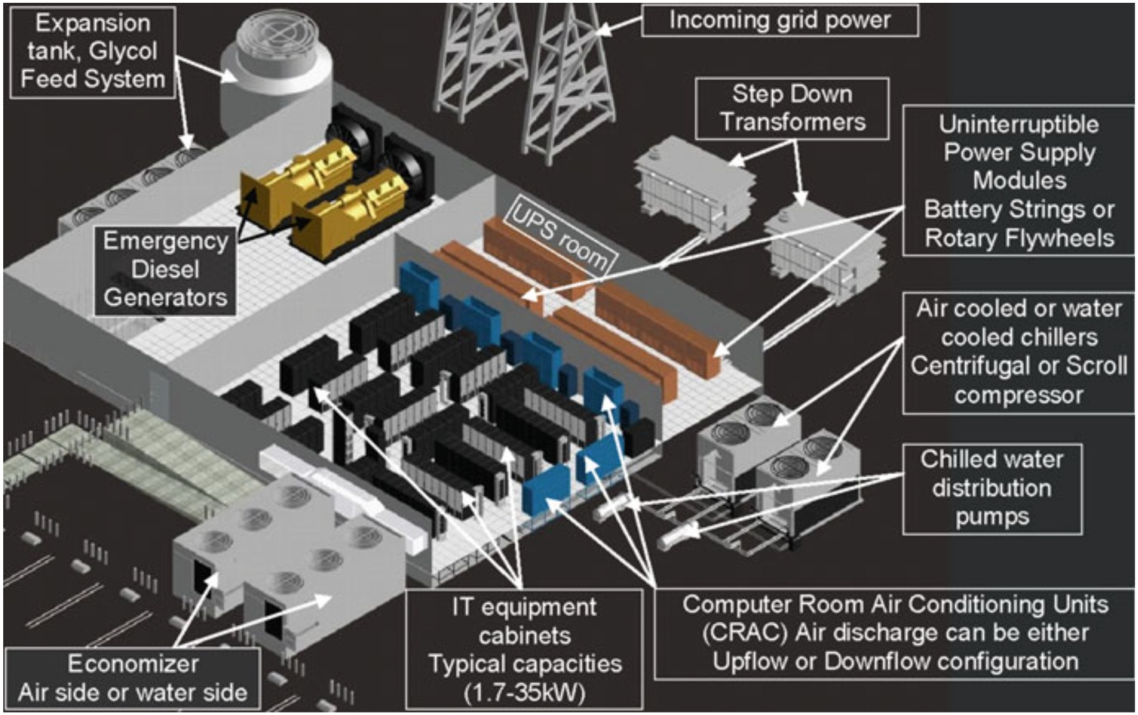
\includegraphics[width=0.65\textwidth]{../figures/joshi2021introduction-figure-01-01.pdf}
%			\vspace{-0.5cm }
		 \caption{(Figure 1.1 in Ref. \cite{joshi2012energy}).}
		\end{figure}
\end{frame}


\begin{frame}
	\frametitle{Seminar 3}
		\begin{itemize}
			\item Michael Donahue, Schneider Electric
%			\item Title: TBD
			\item Date: October 8, 2026
			\item Time: 15:30 (Berkeley Time)
			\item Location: GSPP 150
		\end{itemize}
\end{frame}

    \begin{frame}
        \frametitle{\href{https://datahub.berkeley.edu/user-redirect/git-pull?repo=https://github.com/mtsn-lab/me137-237a&subPath=examples/chipHeatTransfer.ipynb}{Heat Transfer Modeling: Conduction}}
            \begin{figure}
                \centering
                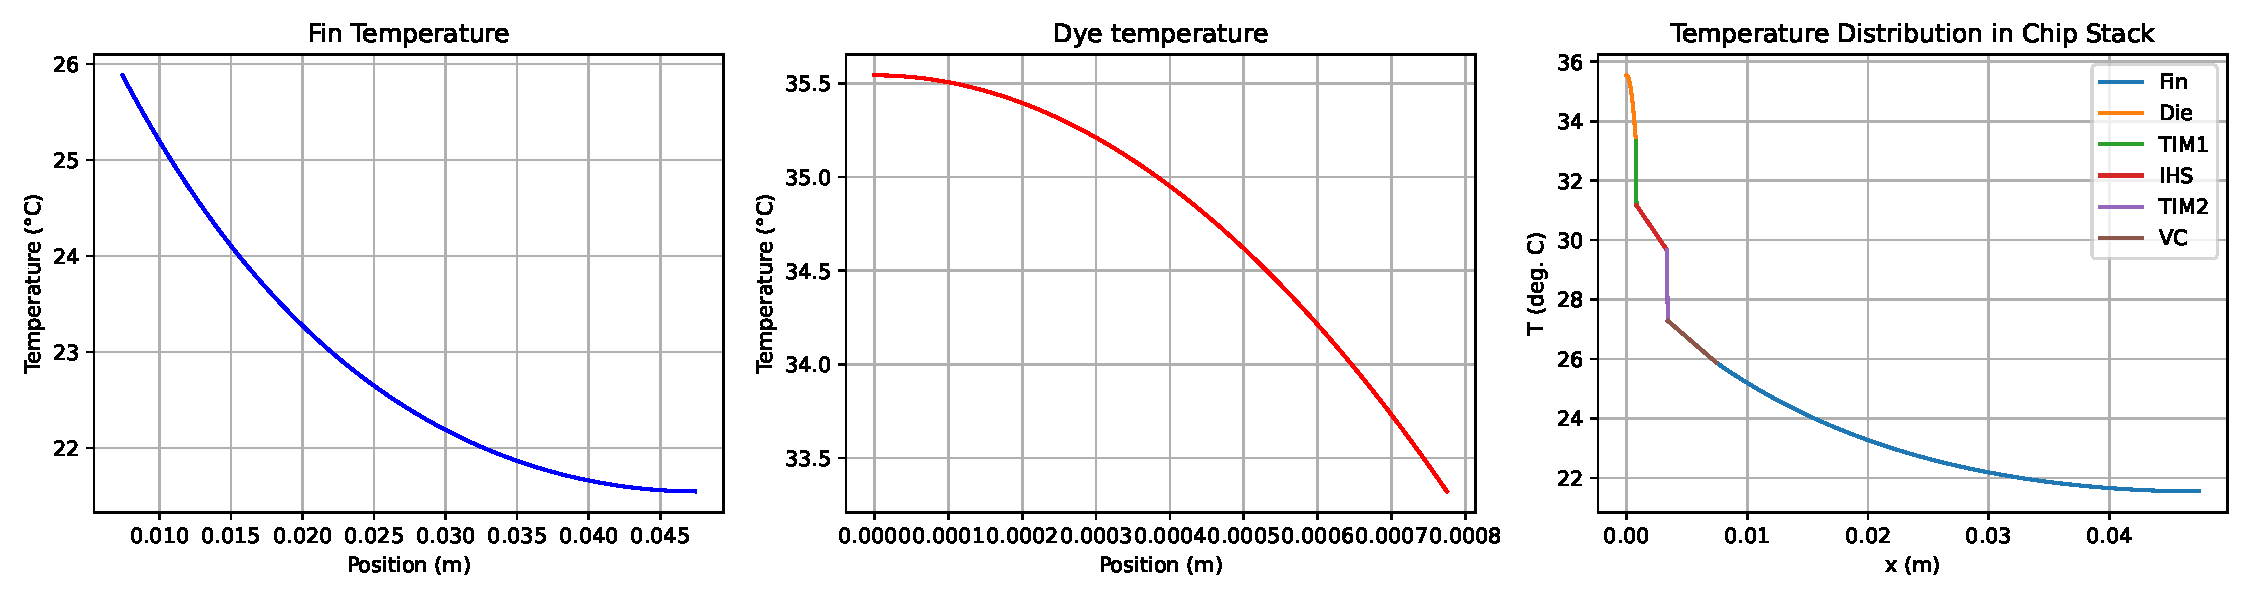
\includegraphics[width=1\textwidth]{../figures/temperature_in_chip_stack.pdf}
                 \caption{Temperature distribution in the chip stack.}
            \end{figure}
    \end{frame}

\begin{frame}
        \frametitle{\href{https://datahub.berkeley.edu/user-redirect/git-pull?repo=https://github.com/mtsn-lab/me137-237a&subPath=examples/heatConduction2dTransientAnalytical.ipynb}{Heat Transfer Modeling: 2D Transient Conduction, Analytical}}			
  		\begin{columns}
			\begin{column}{0.5\textwidth}
				\begin{figure}
					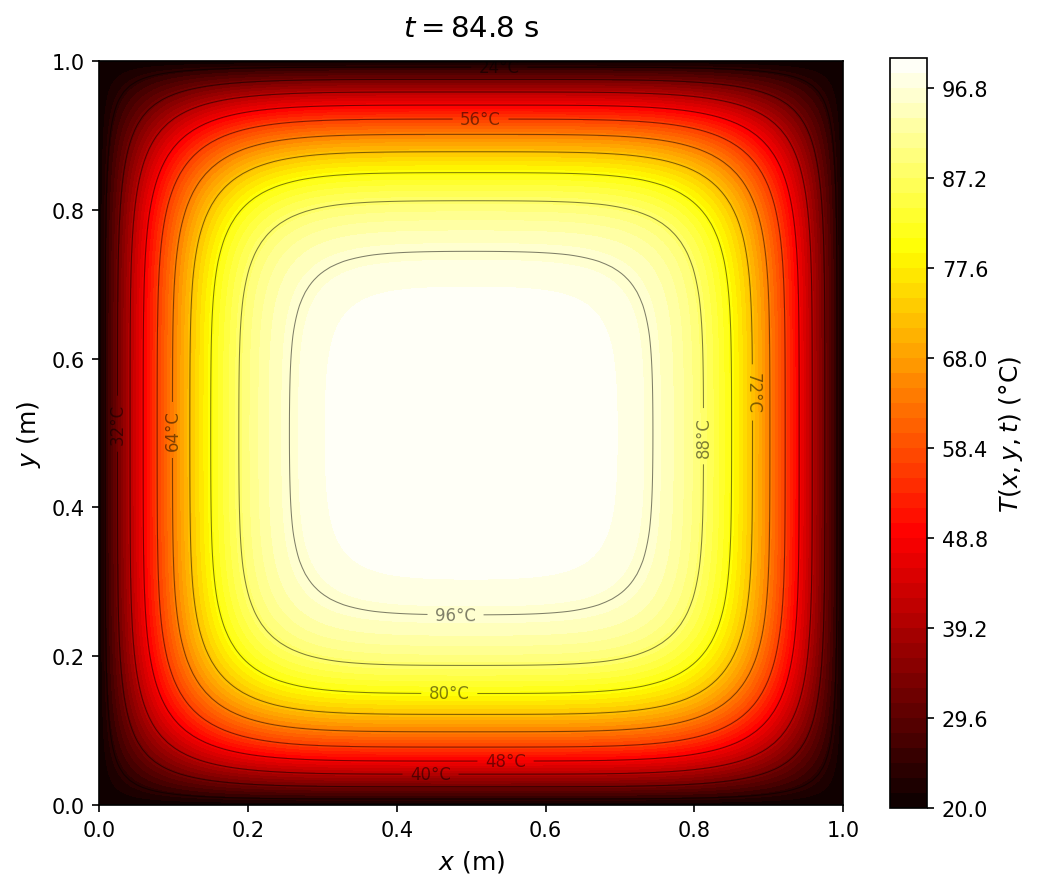
\includegraphics[width=1\textwidth]{../figures/heatConduction2dTransientAnalytical_01.png}
%			\vspace{-0.5cm}
%						 \caption{..}
				\end{figure}
			\end{column}

    			\begin{column}{0.5\textwidth}
				\begin{figure}
					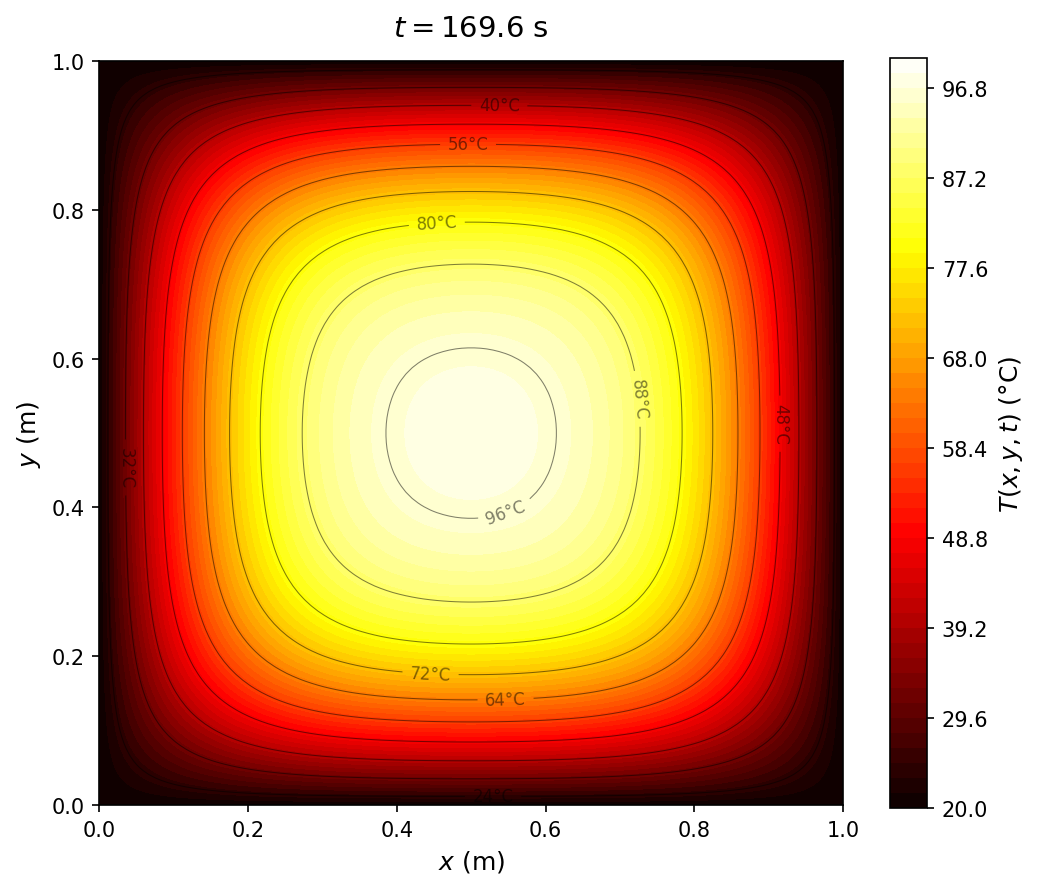
\includegraphics[width=1\textwidth]{../figures/heatConduction2dTransientAnalytical_02.png}
%			\vspace{-0.5cm}
%						 \caption{...}
				\end{figure}
		    	\end{column}
		  \end{columns}
	\end{frame}

    \begin{frame}
        \frametitle{\href{https://datahub.berkeley.edu/user-redirect/git-pull?repo=https://github.com/mtsn-lab/me137-237a&subPath=examples/heatConduction2dTransientNumerical.ipynb}{Heat Transfer Modeling: 2D Transient Conduction, Numerical}}
            \begin{figure}
                \centering
                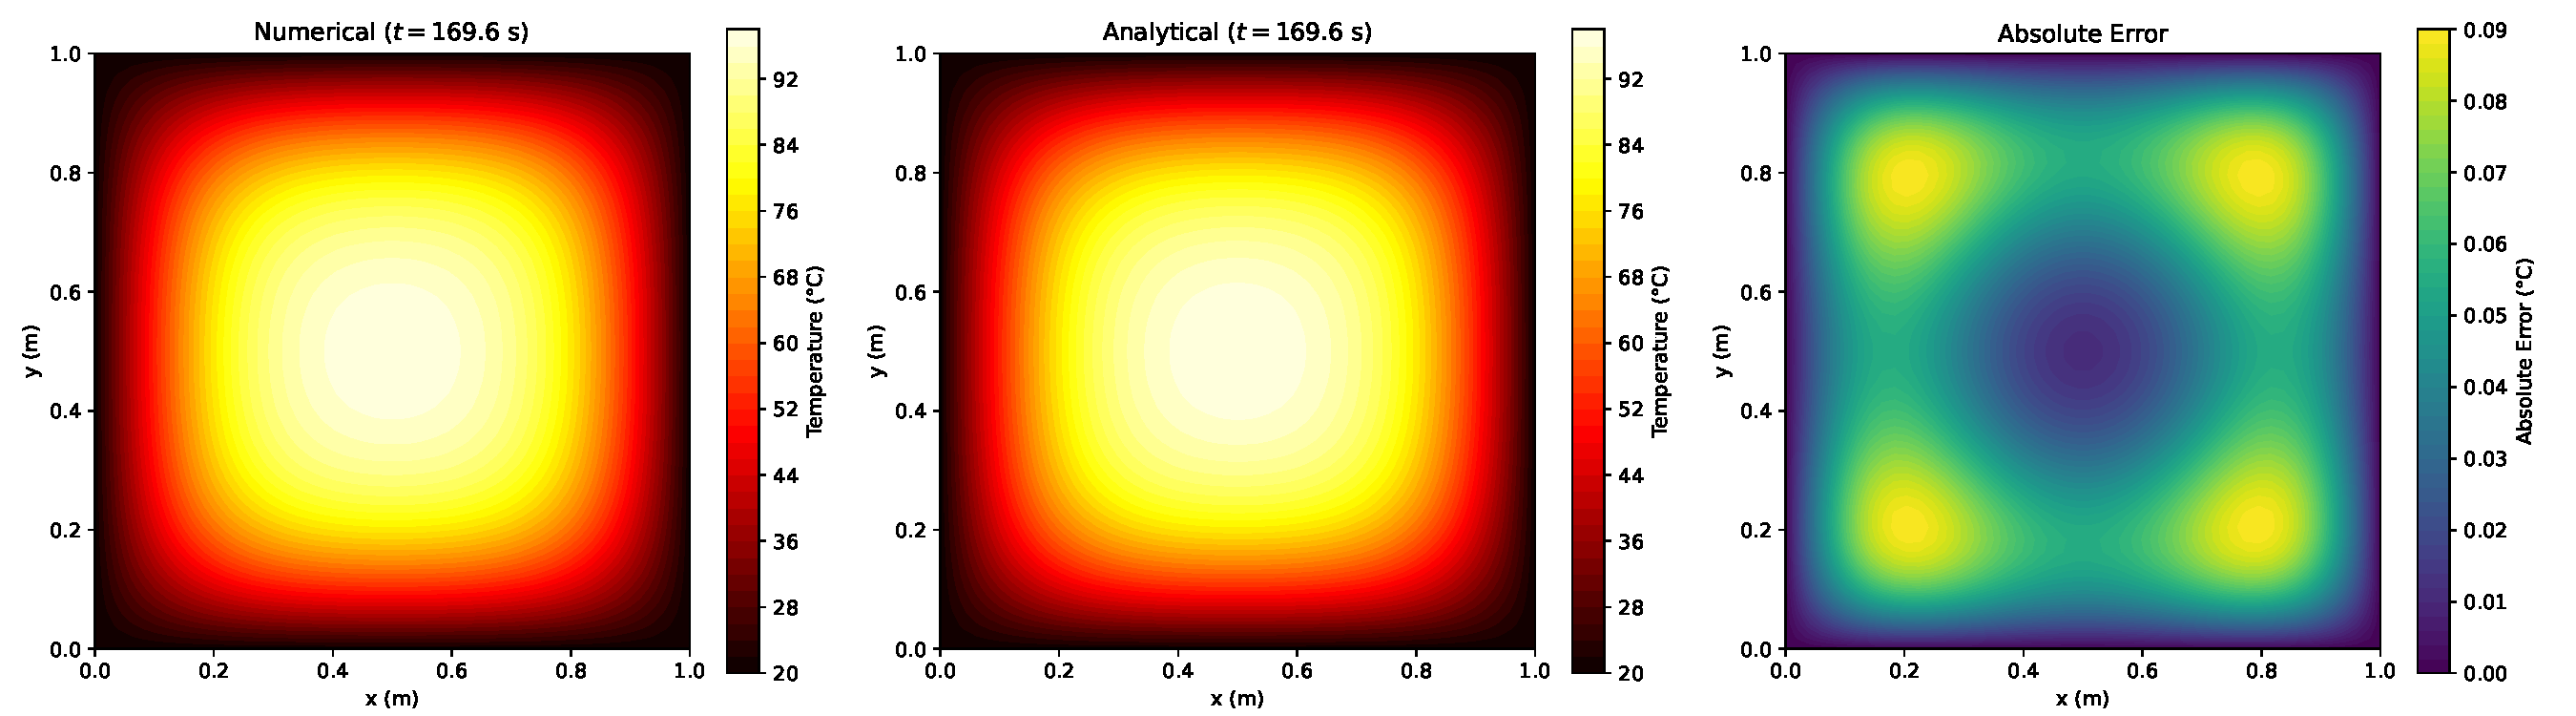
\includegraphics[width=1\textwidth]{../figures/x_y_T_heat_conduction_numerical.pdf}
                 \caption{Analytical vs. numerical solution to the 2D transient heat conduction problem.}
            \end{figure}
    \end{frame}

\begin{frame}
\vspace{-1.5cm}
            \begin{figure}
                \centering
                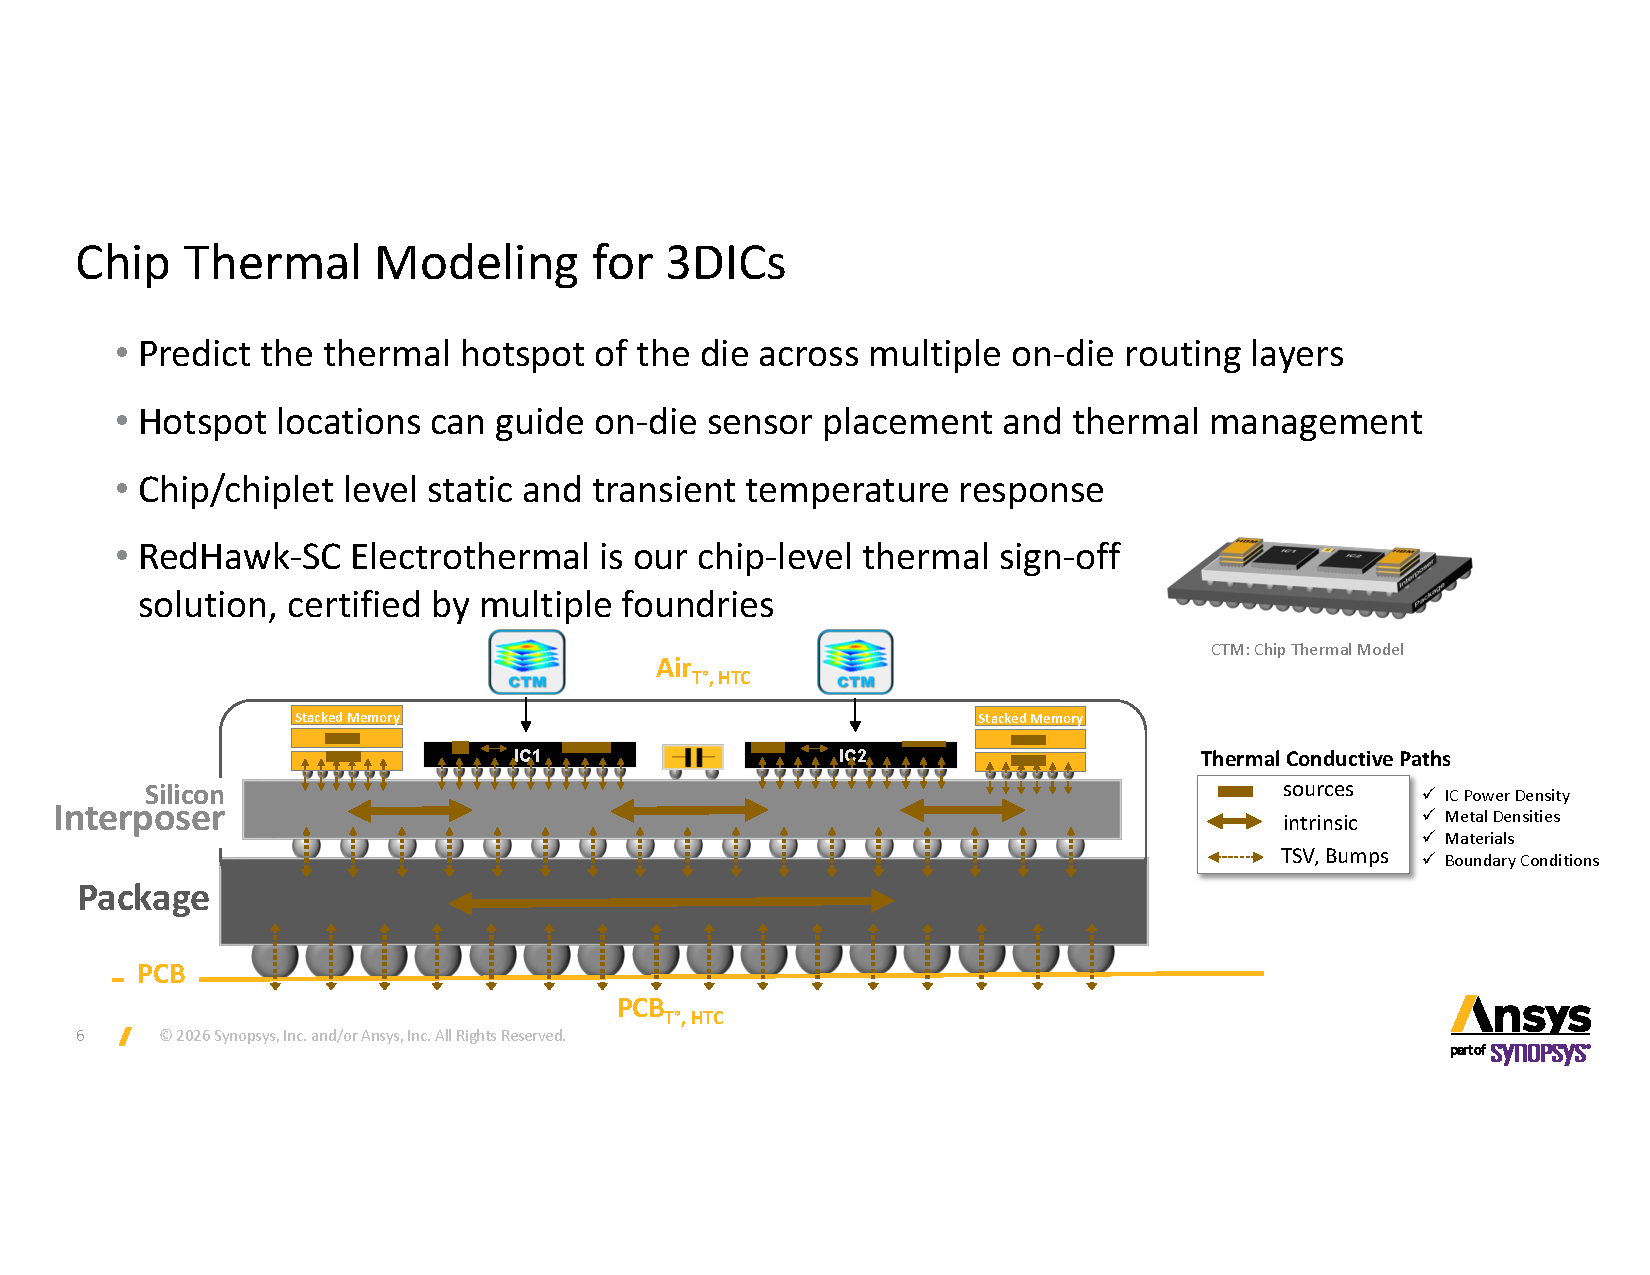
\includegraphics[width=1\textwidth]{../figures/synopsys-chip-thermal.pdf}
%                 \caption{Exact similarity solution vs. numerical solution.}
            \end{figure}
\end{frame}

    
    \begin{frame}
        \frametitle{\href{https://datahub.berkeley.edu/user-redirect/git-pull?repo=https://github.com/mtsn-lab/me137-237a&subPath=examples/heatConduction2dSteadyHeterogeneousNumerical.ipynb}{Heat Transfer Modeling: 2D Steady Conduction, Heterogeneous Material, Numerical}}
            \begin{figure}
                \centering
                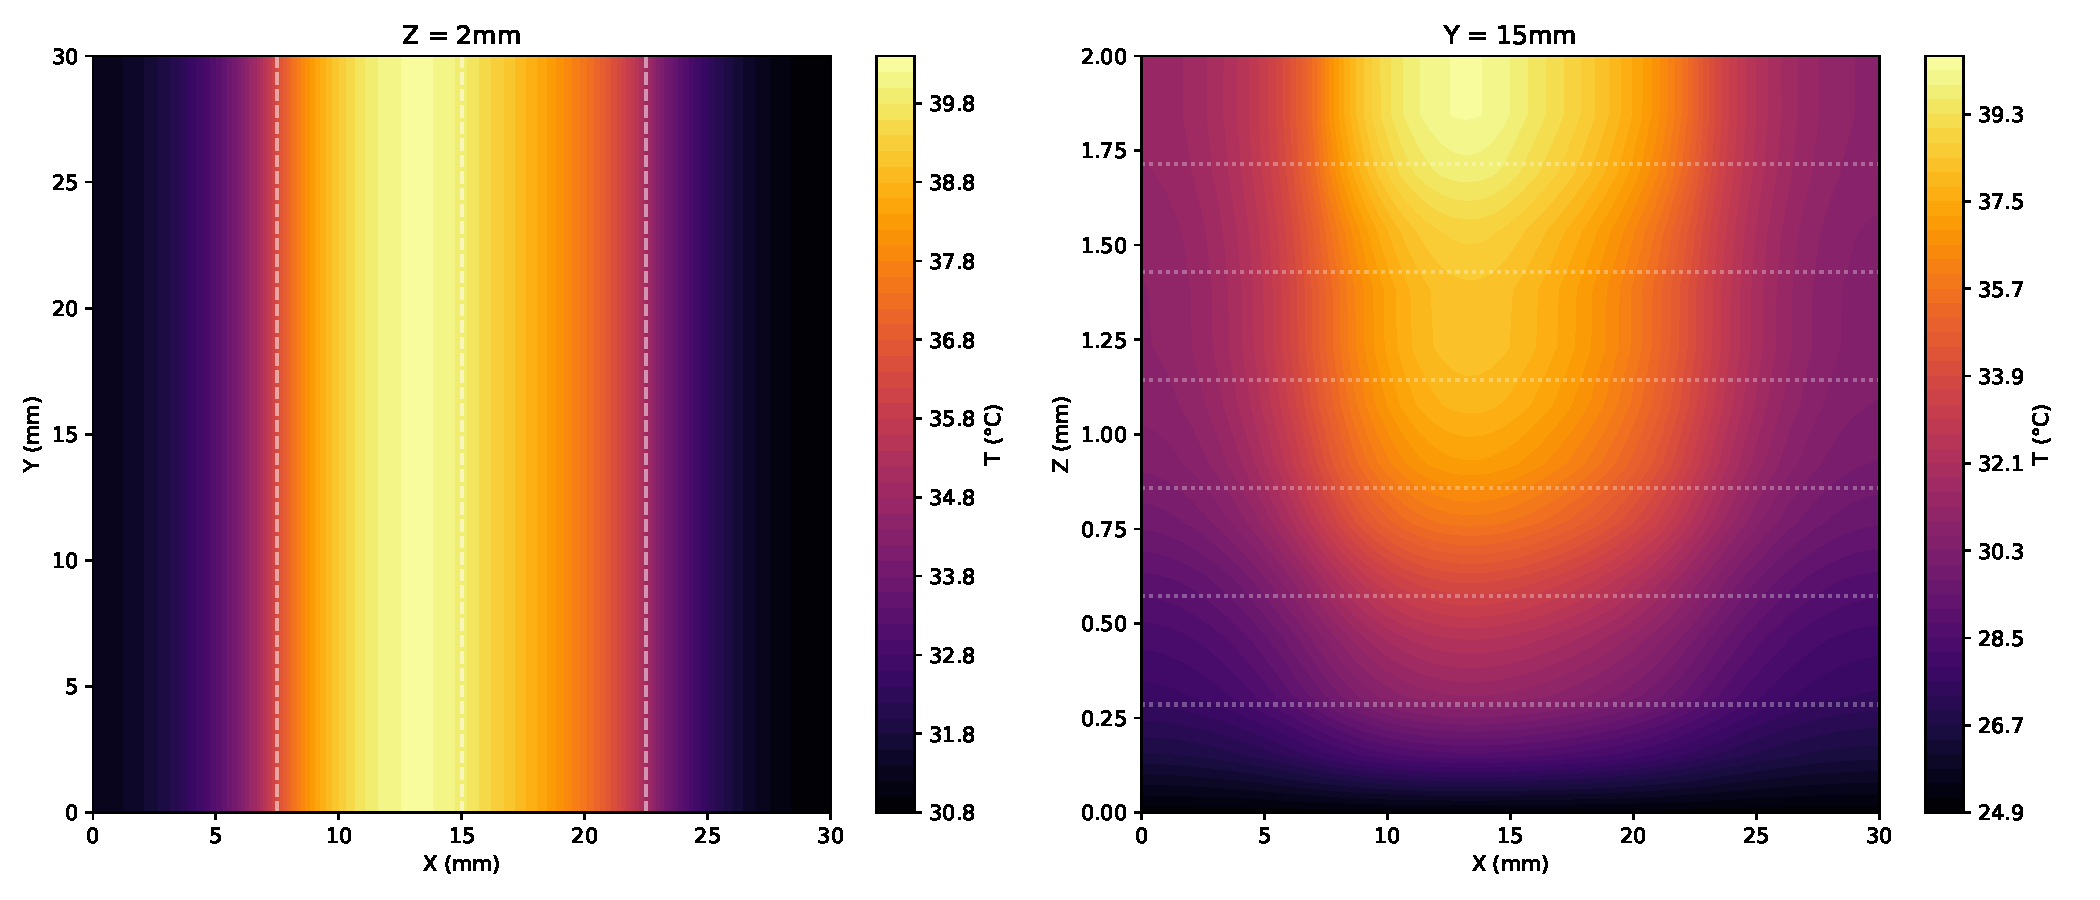
\includegraphics[width=1\textwidth]{../figures/x_y_T_heat_conduction_numerical_2D_heterogeneous_steady.pdf}
                \vspace{-1 cm}
                 \caption{Temperature distribution in 3D IC.}
            \end{figure}
    \end{frame}
    
    

% ------------------------------------------------------------------------------------------------------------------------------------------------------------------------------------
% This is an example for how I link the Jupyter notebook example to the slide I am showing.
% If there is a figure output from the Jupyter notebook, that should be shown here. The Jupyter notebook should be located in me137-237a/examples
% The figure output from the Jupyter notebook should go in the directory me137-237a/lectures/figures

%\begin{frame}
%	\frametitle{\href{https://datahub.berkeley.edu/user-redirect/git-pull?repo=https://github.com/mtsn-lab/me137-237a&subPath=examples/fanLaws.ipynb}{Fan Laws}}
%		\begin{figure}
%			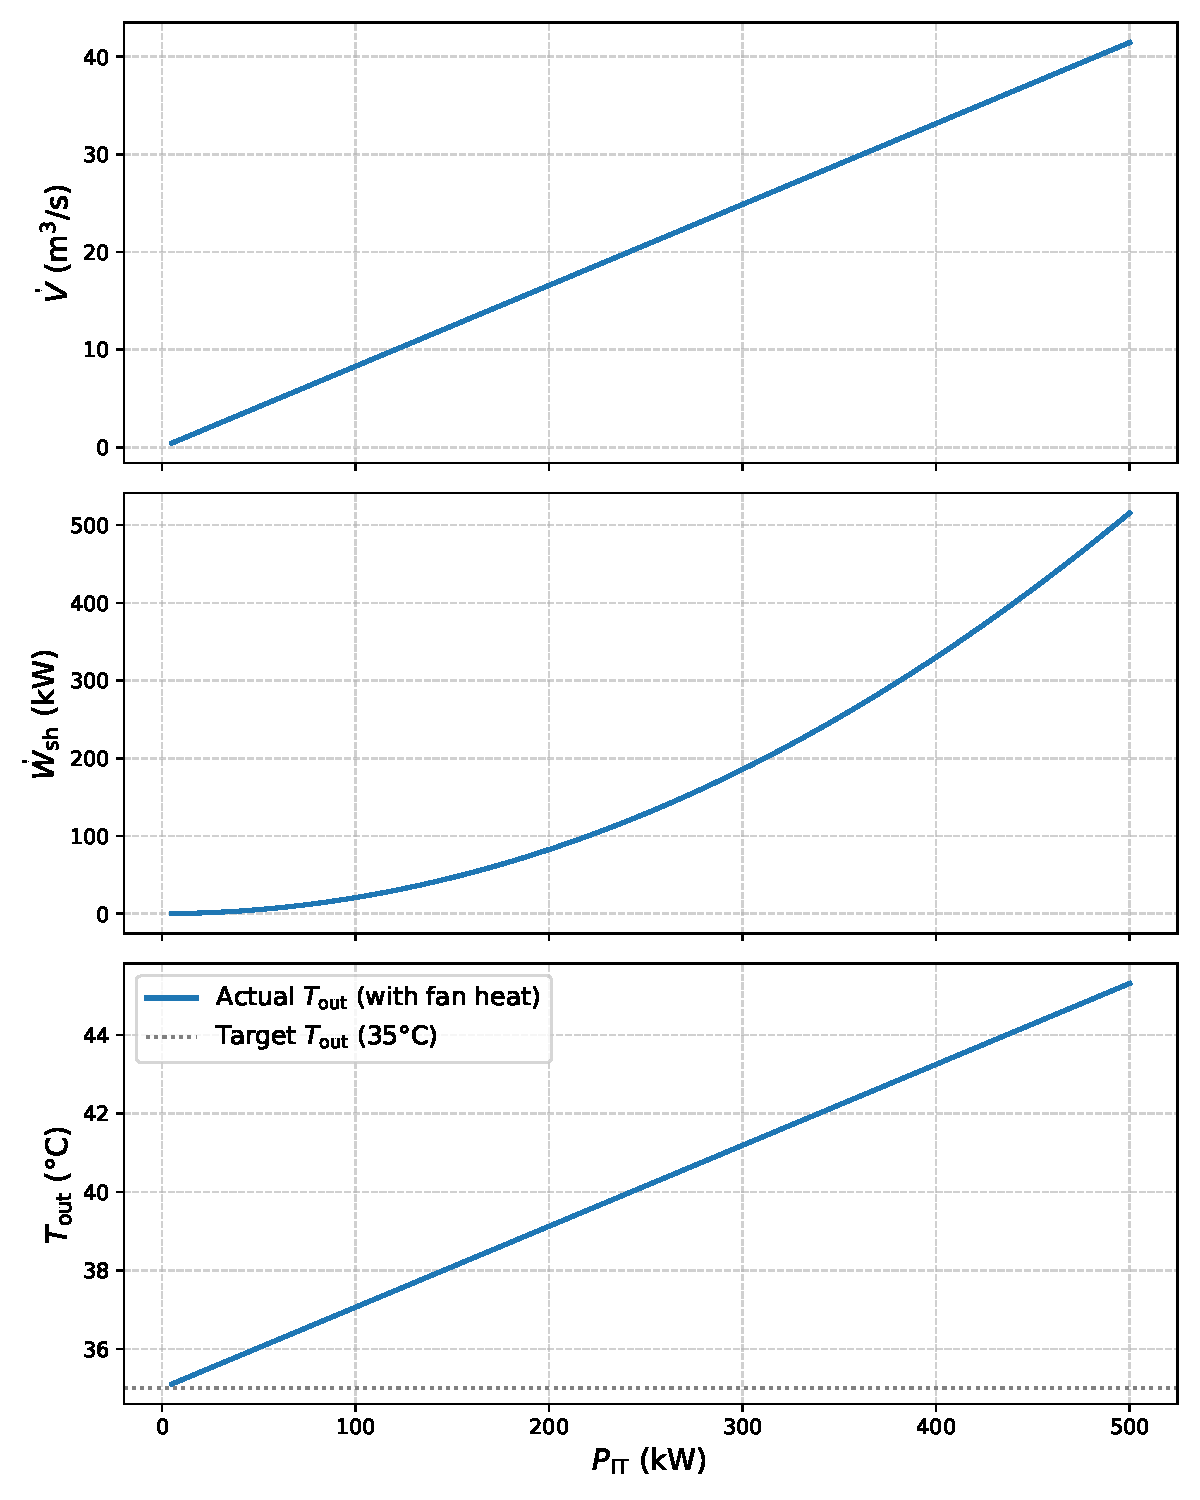
\includegraphics[width=0.4\textwidth]{../figures/rack_cooling_plots.pdf}
%		 \caption{Solution to the Pohlhausen equation. Read his biography \href{https://doi.org/10.1146/annurev.fl.16.010184.000245}{here}.}
%		\end{figure}
%\end{frame}
% ------------------------------------------------------------------------------------------------------------------------------------------------------------------------------------


{
\setbeamertemplate{bibliography item}[text] % Replaces default icons with numbers
	\begin{frame}[allowframebreaks]{References}
		\bibliographystyle{plain}
		\bibliography{../../bibliography}
	\end{frame}
}

}

\end{document}
